\chapter[Sécurité RBAC \& Gamification]{Réalisation : Sécurité RBAC, Gamification \& Sceau Public}
\label{chap:backend_gamification}

\section{Contrôle d'Accès Basé sur les Rôles (RBAC) \& Sécurité JWT}
Dans un environnement étatique sensible, la compartimentation des privilèges est indispensable pour empêcher les accès non autorisés et garantir la traçabilité des opérations d'audit.

\subsection{Matrice des Privilèges \& Hachage Bcrypt}
L'authentification s'appuie sur des jetons \textbf{JSON Web Tokens (JWT)} signés cryptographiquement en \textbf{HMAC-SHA256} avec durée de validité restreinte. Les mots de passe en base sont irréversiblement protégés par l'algorithme \textbf{Bcrypt} (facteur de coût 12). Les rôles sont cloisonnés selon trois niveaux d'autorité :
\begin{itemize}
    \item \textbf{\texttt{Admin} (Super-Admin ANCS)} : Supervision globale des 120 institutions, gestion des comptes utilisateurs, validation des habilitations ministérielles, accès exclusif à la console \texttt{/admin}, édition dynamique du registre des organisations (criticité 1 à 5, contact CSIRT, périmètre surveillé) et activation du mode maintenance.
    \item \textbf{\texttt{Auditor} (Officier RSSI Ministériel)} : Accrédité sur son périmètre ministériel dédié (ex: Ministère des Finances), habilité à déclencher des scans approfondis, à interagir avec l'IA Amina et à exporter les rapports officiels PDF. Toute tentative d'accès à \texttt{/admin} ou de modification du registre étatique est interceptée et bloquée.
    \item \textbf{\texttt{Viewer} (Observateur Public)} : Consultation en lecture seule des scores agrégés et du benchmark international. Les boutons de lancement d'audit, les fonctions de modification et la console d'administration lui sont strictement inaccessibles.
\end{itemize}

\subsection{Écran de Sécurité Souverain HTTP 403 Forbidden sur \texttt{/admin}}
Toute tentative d'accès à la route d'administration par un profil non habilité est stoppée au niveau du routeur Next.js et de l'API FastAPI. L'interface affiche un écran de sécurité haute visibilité rappelant la règle de moindre privilège et journalise la tentative dans l'Audit Trail pour inspection par l'ANCS (Figure \ref{fig:admin_view}).

\subsection{Gestion Dynamique des Organisations \& Privilèges Super-Admin Exclusifs}
Afin de refléter l'évolution des infrastructures publiques sans nécessiter de redéploiement backend, la console d'administration permet la mise à jour en direct du registre des 24 ministères et entités étatiques :
\begin{itemize}
    \item \textbf{Édition directe en ligne} : Modification du niveau de criticité nationale (échelle de 1 à 5 barres selon l'impact souverain), mise à jour de l'adresse de contact d'urgence CSIRT, et enrôlement de nouvelles structures ministérielles.
    \item \textbf{Privilèges strictement réservés au rôle \texttt{admin}} : Ces capacités de mutation sont verrouillées au niveau de l'interface et protégées par des contrôles d'habilitation programmatiques (\texttt{loggedUser.role === "admin"}). Tout profil non-admin est stoppé par une interdiction HTTP 403.
    \item \textbf{Imputabilité \& Audit Trail en temps réel} : Chaque modification ou enrôlement d'institution génère un enregistrement immédiat et infalsifiable dans le flux d'audit (\texttt{LIVE FEED}) avec horodatage à la seconde, garantissant la conformité au Décret-loi n° 2023-17.
\end{itemize}

\begin{figure}[!htbp]
\centering
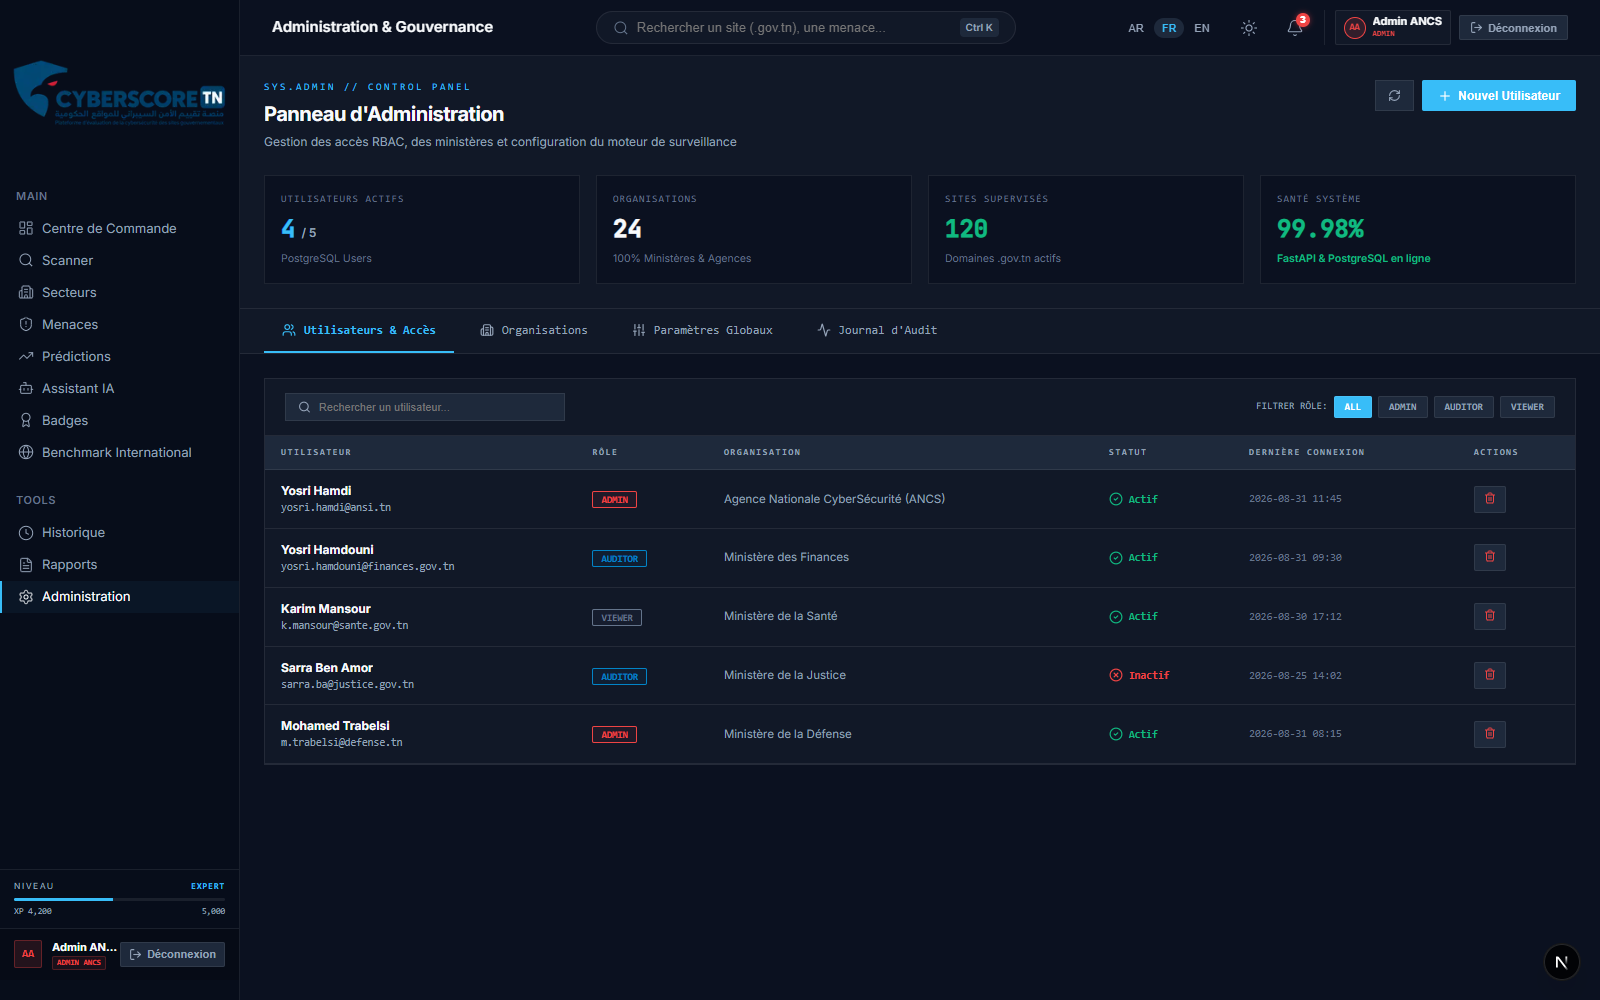
\includegraphics[width=0.70\textwidth]{images/admin.png}
\caption{Console d'administration sécurisée et écran de protection RBAC HTTP 403 Forbidden}
\label{fig:admin_view}
\end{figure}

\section{Module de Gamification Institutionnelle \& Niveaux RSSI}
Afin d'inciter les départements ministériels à corriger activement leurs vulnérabilités, CyberScore TN intègre un système d'émulation basé sur l'attribution de points d'expérience (\textbf{XP}).

\subsection{Paliers de Compétence SOC}
L'officier RSSI progresse à travers cinq échelons de reconnaissance affichés dans la barre latérale :
\begin{enumerate}
    \item \textbf{Niveau 1 -- DÉBUTANT ($0 - 1\,000$ XP)} : Prise en main et premiers scans réalisés.
    \item \textbf{Niveau 2 -- INTERMÉDIAIRE ($1\,000 - 2\,000$ XP)} : Audits réguliers du périmètre ministériel.
    \item \textbf{Niveau 3 -- AVANCÉ ($2\,000 - 3\,500$ XP)} : Résolution active des alertes critiques et durcissement SSL/DNS.
    \item \textbf{Niveau 4 -- EXPERT ($3\,500 - 5\,000$ XP)} : Maintien continu du parc au Grade A/A+ et exports officiels.
    \item \textbf{Niveau 5 -- ÉLITE SOC ($5\,000+$ XP)} : Posture exemplaire sur l'ensemble des 16 piliers d'audit.
\end{enumerate}

\subsection{Référentiel des 12 Badges d'Excellence}
Le système évalue automatiquement les métriques enregistrées en base pour attribuer douze trophées officiels aux officiers de sécurité et aux organismes :

\begin{table}[!htbp]
\centering
\caption{Catalogue officiel des 12 badges d'émulation de CyberScore TN}
\label{tab:gamification_badges}
\begin{singlespace}
\footnotesize
\renewcommand{\arraystretch}{1.08}
\begin{tabularx}{\textwidth}{l l c X}
\toprule
\textbf{Code Badge} & \textbf{Intitulé Officiel} & \textbf{XP} & \textbf{Condition de Déblocage Vérifiée} \\
\midrule
\texttt{FIRST\_SCAN} & Premier Pas & +100 & Réalisation du premier audit sur un portail public. \\
\texttt{WARRIOR} & Guerrier de la Sécurité & +250 & Audit complété sur dix domaines étatiques distincts. \\
\texttt{CLEAN\_SWEEP} & Nettoyage Total & +300 & Élimination de toute vulnérabilité critique sur le parc. \\
\texttt{SSL\_CHAMP} & Champion TLS & +250 & Note parfaite de 100/100 sur le pilier SSL/TLS (TLS 1.3). \\
\texttt{HEADERS\_HERO} & Héros des Headers & +250 & Note de 100/100 sur les en-têtes HTTP de sécurité. \\
\texttt{DNS\_GUARD} & Gardien DNS & +200 & Validation DNSSEC et conformité DMARC (\texttt{p=reject}). \\
\texttt{CENTURION} & Centurion du SOC & +500 & Atteinte du seuil de 100 sessions d'audit conduites. \\
\texttt{SECTOR\_LEAD} & Leader Sectoriel & +400 & Première place obtenue au classement du secteur ministériel. \\
\texttt{FAST\_PATCH} & Chasseur de Failles & +350 & Résolution vérifiée d'une faille critique sous 24 heures. \\
\texttt{TRUST\_SEAL} & Sceau de Confiance & +400 & Attribution officielle du label de confiance 3 étoiles. \\
\texttt{VELOCITY} & Audit Véloce & +150 & Audit Standard exécuté avec succès en moins de 5 secondes. \\
\texttt{PERFECTION} & Perfection Nationale & +1\,200 & Score d'audit parfait de 100/100 en mode Approfondi. \\
\bottomrule
\end{tabularx}
\end{singlespace}
\end{table}

La Figure \ref{fig:badges_view} illustre la console d'émulation présentant les paliers de points d'expérience et l'état de déblocage des trophées pour l'organisme audité.

\begin{figure}[!htbp]
\centering
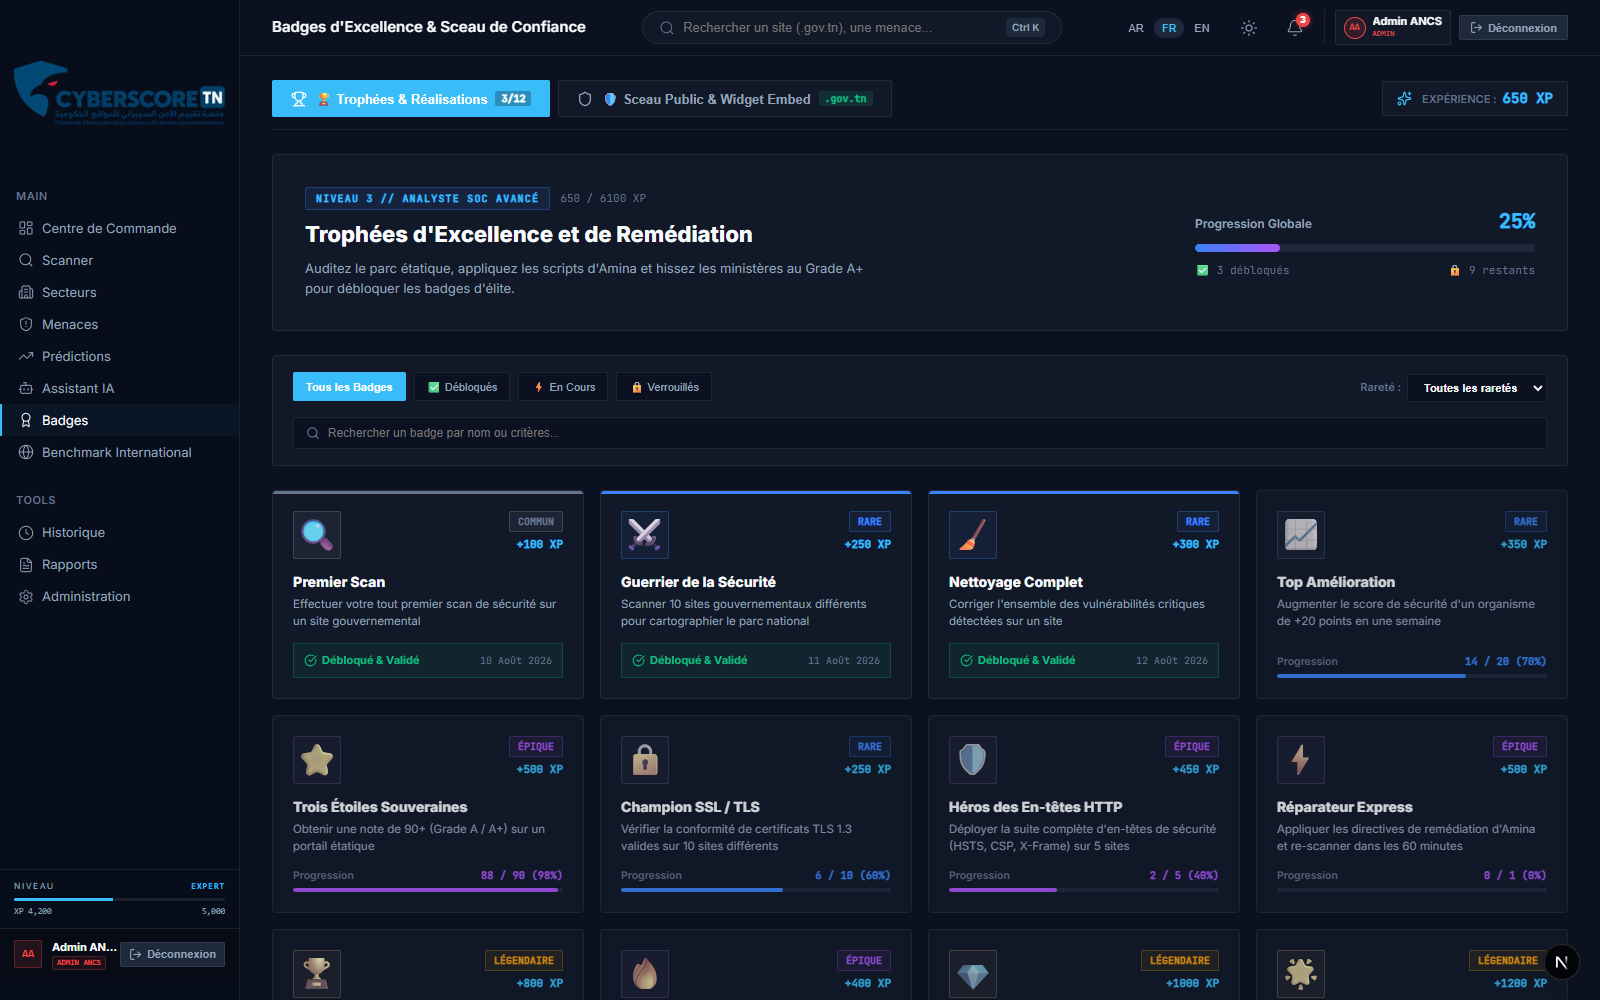
\includegraphics[width=0.70\textwidth]{images/badges.png}
\caption{Centre d'émulation institutionnelle et catalogue interactif des 12 badges SOC}
\label{fig:badges_view}
\end{figure}

\section{Sceau Public de Confiance \& Widget SVG Sécurisé}
Pour valoriser les efforts de mise en conformité auprès du grand public, les organismes atteignant l'excellence peuvent exporter le \textbf{Sceau Numérique de Confiance CyberScore TN} :
\begin{itemize}
    \item \textbf{Widget Vectoriel Dynamique} : Badge SVG auto-actualisé affichant le grade souverain (\texttt{A+}, \texttt{A}, \texttt{B}) et le label d'étoiles ($\star\star\star$).
    \item \textbf{QR Code Anti-Fraude} : Chaque badge embarque un QR code dynamique généré côté client et serveur pointant vers l'URL officielle de vérification cryptographique (\texttt{https://cyberscore.tn/[locale]/verify/[domaine]}), interdisant l'usage frauduleux d'une image statique par un portail non certifié.
    \item \textbf{Variantes d'Intégration} : Cartouche complet institutionnel (armoiries, note, étoiles et QR code), bouclier vertical (\textit{Shield}) et bandeau compact (\textit{Pill}) pour pieds de page.
\end{itemize}

\section{Portail Souverain de Vérification \& Hygiène Numérique Citoyenne}
Afin de concrétiser la vérification par smartphone accessible à tout citoyen, nous avons conçu la route dynamique \texttt{/[locale]/verify/[domain]} :
\begin{enumerate}
    \item \textbf{Architecture Trilingue Réactive} : Prise en charge native de l'Arabe (\textit{RTL}), du Français et de l'Anglais (\textit{LTR}) avec commutation instantanée sans rechargement de page et protection stricte contre les conflits d'hydratation (\texttt{suppressHydrationWarning}).
    \item \textbf{Cloisonnement Défensif TLP:AMBER+STRICT} : L'usager public accède à la certification macroscopique, au score et aux étoiles sans pouvoir consulter les données offensives d'audit. Le rapport technique complet de 7 pages (détaillant les CVE, ports ouverts et snippets de correction) ainsi que le déclencheur de re-scan sont strictement verrouillés derrière une authentification forte réservée aux RSSI accrédités de l'ANCS.
    \item \textbf{Carrousel Héroïque d'Hygiène Numérique} : Un slider interactif animé à rotation automatique (5,5s) avec pause au survol présente les 4 réflexes vitaux de cyber-vigilance : vérification du cadenas HTTPS et du domaine officiel \texttt{.gov.tn}, alerte anti-phishing et faux SMS, activation de l'authentification à double facteur (2FA), et signalement d'urgence auprès du CERT National (ANCS) via le numéro d'urgence \texttt{71 843 200}.
\end{enumerate}

\section{Modélisation des Menaces \& Résilience Face au Phishing (Anti-Phishing)}
Une question déterminante de sécurité offensive s'impose lors de l'évaluation du système : \textit{« Un cybercriminel peut-il capturer le QR code officiel d'un ministère et le publier sur son faux site pour abuser la confiance des citoyens ? »}

Notre réponse technique neutralise cette menace par \textbf{trois lignes de défense coordonnées} basées sur le principe de \textbf{Liaison de Domaine (Domain Binding)} :
\begin{enumerate}
    \item \textbf{Le Piège de Non-Concordance de Domaine (Domain Mismatch Trap)} : Le QR code encode exclusivement l'URL officielle certifiée de l'État (\texttt{cyberscore.tn/verify/sante.gov.tn}). Lorsque la victime scanne le QR code volé depuis un faux portail (\texttt{sante-fake-tunisie.com}), son smartphone ouvre la page souveraine de l'ANCS affichant en gros caractères officiels : \textit{« Cette attestation appartient exclusivement au Ministère de la Santé (sante.gov.tn) »}. La victime constate la divergence flagrante avec l'adresse affichée sur son ordinateur : l'escroquerie est démasquée en une seconde. La capture du QR code devient ainsi le piège qui confond l'attaquant.
    \item \textbf{Ancrage d'Infrastructure Souveraine .tn \& TunTrust} : Un fraudeur ne peut enregistrer de domaine officiel sous la zone étatique \texttt{.tn} (régulée par l'ATI et l'ANCS), ni obtenir un certificat serveur officiel TunTrust sous le backbone AS2609. S'il tente de faire auditer son faux domaine sur la plateforme CyberScore TN, les 6 moteurs de scan passif détectent immédiatement l'absence d'infrastructure nationale et lui attribuent la note éliminatoire de \textbf{Grade F (0/100) — DOMAINE SUSPECT}.
    \item \textbf{Validation Dynamique d'Origine (HTTP Referer \& Hostname)} : Le widget JavaScript (\texttt{BadgesClient.tsx}) vérifie à l'exécution le nom d'hôte (\texttt{window.location.hostname}) et l'en-tête \texttt{Referer}. En cas d'appel depuis un domaine non répertorié dans la base nationale, le serveur révoque l'affichage du sceau de confiance au profit d'un avertissement d'invalidité.
\end{enumerate}

